\clearpage{}
\section{Closure typing}
\label{System:Closure}

Leroy's \emph{closure-typing} \cite{leroy:polymorphic-type-inference, leroy:polymorphic-typing} is a system for modeling data sharing due to the inclusion of free variables in the bodies of functions. 
We use closure typing as an alternate solution to the problem of polymorphic update, as well as to reason about the sharing properties of regions. 

Consider the following function:

\code{
	$\iaddT = \lambda x. \ \lambda y. \ (x + y, \ x)$
}

If we take addition $(+)$ to operate on values of type $\iInt$, then we could give $\iaddT$ the following type:

\code{
	$\iaddT :: \iInt \to \iInt \to \iPair \ \iInt \ \iInt$
}

If we then partially apply $\iaddT$ to the value 5, the first argument of its type is satisfied and we end up with a function that accepts an integer and produces a pair:

\code{
	$\iaddFive :: \iInt \to \iPair \ \iInt \ \iInt$ \\
	$\iaddFive = \iaddT \ 5$ \\
}

$\iaddFive$ can be further applied to yield the pair, but what happened to the first value we provided? Assume  evaluation proceeds via template instantiation after the pure lambda calculus. In this case we could reason that the argument $5$ was bound to the formal parameter $x$ and then substituted into the body of the outer lambda abstraction, that is:

\code{
	$\iaddFive$ 
	& $\longrightarrow \iaddT \ 5$	\\
	& $\longrightarrow (\lambda x. \ \lambda y. \ ( x + y, \ x)) \ 5$ \\
	& $\longrightarrow \lambda y. \ (5 + y, \ 5)$ 
}

This call-by-name reasoning is applicable to a pure language such as Haskell, but as we intend to use
destructive update we must take a more operational approach. If we instead consider an implementation based on super-combinators \cite{hughes:thesis}, we would treat $\iaddT$ as a single supercombinator, and the partial application $(\iaddT \ 5)$ as the construction of a thunk containing pointers to the supercombinator code and argument value:

\begin{center}
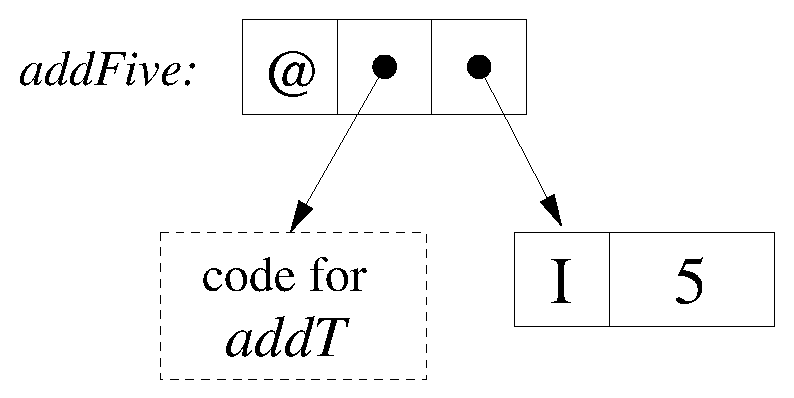
\includegraphics[scale=0.4]{2-System/fig/closure-super.eps}
\end{center}

When $\iaddFive$ is applied to its final argument, the code for $\iaddT$ is called directly. $\iaddT$'s first argument comes from the thunk, and the second is supplied by the application. This is how DDC operates.

With this system, every use of $\iaddFive$ shares the same `5' object. Using region annotations on data types and closure annotations on functions\footnote{We modify Leroy's syntax for closures to be similar to the one used for effects.}, we give $\iaddFive$ a type which makes the sharing explicit.

\code{
	$\iaddFive$ 
	& $::$		& $\forall r_1 \ r_2 \ r_3$ \\
	& $.$		& $\iInt \ r_1 \lfuna{c_1} \iPair \ r_2 \ (\iInt \ r_3) \ (\iInt \ r_4)$ \\
      	& $\rhd$	& $c_1 = x : \iInt \ r_4$ \\
}

On the left of the function arrow, the argument type $\iInt \ r_1$ says that $\iaddFive$ accepts an integer from a region which we name $r_1$. On the right of the arrow, we see that the function produces a pair of integer components. As $r_3$ is quantified, we infer that the first component has been freshly allocated into a new region (addition returns a fresh result). The data constructor representing the pair is also fresh, so $r_2$ is quantified as well. On the other hand, $r_4$ is \emph{not} quantified, which indicates that the second component of the pair will be in the same region each time $\iaddFive$ is called. 

The closure variable $c_1$ attached to the function arrow indicates that the definition of $\iaddFive$ creates a shared value, and the term $x : \iInt \ r_4$ records its type. The ``$x :$'' portion of $x : \iInt \ r_4$ is called the \emph{closure tag}, and we treat it as an operator that lifts the type term $\iInt \ r_4$ into a closure term. In this example, the variable $x$ corresponds to the occurrence that is free in the innermost lambda-abstraction in the definition of $\iaddFive$. For the types of primitive functions such as data constructors, although there is no associated source code we still use names such as $x, y, z$ for consistency. 

Note that our type system tracks variable names such as $x$ as a notational convenience, but does not make use of them for checking purposes. We have found it useful for such variables to be included in the types presented to the user, as without them it can be very difficult to determine why an inferred type signature includes a particular closure term. However, if desired we could replace all such variables with an underscore to indicate they are ignored by the type system proper.

% --------------------
\subsection{Dangerous type variables}
\label{System:Closure:dangerous}

In \cite{leroy:polymorphic-typing} Leroy defines dangerous variables to be the ones that are free in a live reference type. For Disciple this is equivalent to being free under a mutable type constructor.

Consider the following type:

\code{
	$\ithing$	
	& $::$		& $\iMaybe \ r_1 \ (a \to a)$ \\
	& $\rhd$	& $\iMutable \ r_1$
}

\quad with

\code{
	\mc{4}{$\kdata \ \iMaybe \ r_1 \ a$} \\
		& $=$	& $\iNothing$ \\
		& \ $|$	& $\iJust \ \{ x :: a \}$
}

In the type of $\ithing$, $a$ is dangerous because it corresponds to a value that we are able to update at runtime. For example, the following code creates a $\iJust$ constructor containing the function $\iid$, updates it to hold the less general function $\isucc$, then tries to apply that function to a string. This example is similar to one from \S\ref{System:PolyUpdate}, except that we are using the Disciple projection syntax to update the mutable object. The term $\ithing \ \odot_{\#} \ x$ creates a reference to the $x$ field in the $\iJust$ constructor. If we view references as being akin to pointers, then $\ithing \ \odot_{\#} \ x$ has a similar meaning to the C expression \texttt{\&(thing.x)}. Projections are discussed further in \S\ref{System:Projections}. 

\clearpage{}
Once the reference is created, we use the $:=_{\#}$ operator to update the field (via the reference):

\code{ 
	$\kdo$	& $\ithing$	& $= \iJust \ \iid$ 
		\\[1ex]
		& $thing \ \odot_{\#} \: x$	
				& ${:=_{\#}} \ \isucc$ 
		\\[1ex]
		& $\itrouble$	& $= \kcase \ \ithing \ \kof \ {\iJust \ f \to \ f \ ``\texttt{die!}"}$
}

When generalising the type of $\ithing$ we must hold $a$ monomorphic. If we were to give it the following polymorphic type, then the above code would pass the type checker, but would have an undefined result at runtime.

\code{
	$\ithing_{\ibad}$	
	& $::$		& $\forall a. \ \iMaybe \ r_1 \ (a \to a)$ \\
	& $\rhd$	& $\iMutable \ r_1$
}

In general, to determine the dangerous variables in a type we must inspect the definitions of the data types involved. 

For example, the following type has three separate region variables, which gives us three places to attach mutability constraints:

\code{
	\mc{3}{$\kdata \ \iTwoThings \ r_1 \ r_2 \ r_3 \ a \ b$} \\
	& $=$	& $\iThingOne \ (\iMaybe \ r_2 \ a)$ \\
	& $\ |$	& $\iThingTwo \ (\iMaybe \ r_3 \ b)$
}

Here is an example signature that uses $\iTwoThings$:

\code{
	$\ifoo$	& :: 		& \mc{3}{$\iTwoThings \ r_4 \ r_5 \ r_6 \ (d \to \iInt \ r_7) \ (\iChar \ r_8)$} \\
		& $\rhd$	& $\iConst \ r_4$	\\
		& , 		& $\iMutable \ r_5$	\\
		& ,		& $\iConst \ r_6$
}

In this case, as $r_5$ is mutable we must hold $d$ and $r_7$ monomorphic. Note that region, effect and closure variables can be dangerous as well. As $r_5$ is mutable we cannot generalise $r_7$ because the associated $\iMaybe$ object might be updated to hold a function that does not allocate a fresh return value. On the other hand, we can allow $r_8$ to be polymorphic as $r_6$ is constant. If $r_4$ was mutable then all of $r_5$, $r_6$, $d$, $r_7$ and $r_8$ would have to be monomorphic, because this would let us update either of the $\iThing$ objects to hold a different $\iMaybe$.

A formal description of which variables are dangerous is given in \S\ref{Inference:Language}.


% ----------------
\subsection{Closure typing and hidden communication}
\label{System:Closure:masking}

Consider the following function, also from \cite{leroy:polymorphic-typing}:

\code{
	\mc{4}{$\imakeGetSet \ x$} \\
	& $\kdo$	& $\iref$	& $= \inewRef \ x$ \\
	&		& $\iget \ ()$	& $= \ireadRef \ \iref$ \\
	&		& $\iset \ z$	& $= \iwriteRef \ \iref \ z$ \\
	&		& \mc{2}{$\iPair \ \iget \ \iset$}
}

This function allocates a reference to the supplied value $x$, and then returns a pair of functions to get and set the value in the reference. 

\clearpage{}
In Disciple, without closure information and before generalisation, the type of $\imakeGetSet$ is:

\code{
	$\imakeGetSet$ 
	& $::$		& \mc{2}{$a \to \iPair \ r_1 \ (() \lfuna{e_1} a) \ (a \lfuna{e_2} ())$} \\
	& $\rhd$	& $e_1$		& $\tme \iRead \  r_2$ \\
	& $,$		& $e_2$		& $\tme \iWrite \ r_2$ \\
	& $,$		& \mc{2}{$\iMutable \ r_2$}
}

There are two problems with this type. Firstly, as $r_2$ is not mentioned in the body (or the type environment), the read and write effects will be masked as per \S\ref{System:Effects:masking}. This is invalid because the order in which these applications take place at runtime certainly matters, so they must retain their effect terms. Secondly, if we were to allow $a$ to be generalised then we would have an unsound system once again. 

For example:

\code{
	$\imakeGetSet_{\ibad}$ 
	& $::$		
	& \mc{2}{$\forall a \ r_1. \ a \to \iPair \ r_1 \ (() \to a) \ (a \to ())$} \\
}

\code{
	\mc{4}{$\ibroken \ ()$} \\
	& $\kdo$	& $\igetset$	& $= \imakeGetSet_{\ibad} \ \iid$ 
	\\[1ex]
	&		& $\isetTwo$	& $= \isnd \ \igetset$ \\
	&		& \mc{2}{$\isetTwo \ \isucc$}
	\\[1ex]
	&		& $\igetTwo$	& $= \ifst \ \igetset$ \\
	&		& \mc{2}{$\igetTwo \ () \ ``\texttt{die!}"$}
}


By allowing the mutable object $\iref$ to be free in the closure of the get and set functions, we have created a communication channel between them that is not visible in their types. This is not a problem in itself, but the addition of let-polymorphism allows each function to gain a different understanding of what type of data is being sent across the channel. Note that with the bad type for $\imakeGetSet$, the inferred type of $\igetset$ includes a quantifier for $b$:

\code{
	$\igetset$	:: $\forall b. \ \iPair \ r_1 \ (() \to (b \to b)) \ ((b \to b) \to ())$ \\
}

As we have used a let-binding to define $\igetTwo$ and $\isetTwo$, the types of the two components are re-generalised and we end up with:

\code{
	$\igetTwo$	:: $\forall c. \ () \to (c \to c)$ \\
	$\isetTwo$	:: $\forall d. \ (d \to d) \to ()$ \\
}

The use of $\isetTwo$ updates the shared reference to contain a function, $\isucc$, that only accepts integers. Unfortunately, with $\igetTwo$ we can then read it back and pretend that it accepts a string.

Adding closure information to our types remedies this problem. Here is the new type of $\imakeGetSet$, with closure information, and before generalisation:

\code{
	$\imakeGetSet$ 
	& $::$		& \mc{2}{$a \to \iPair \ r_1 \ (() \lfuna{e_1 \ c_1} a) \ (a \lfuna{e_2 \ c_2} ())$} \\
	& $\rhd$	& $e_1$		& $\tme \ \iRead \  r_2$ \\
	& $,$		& $e_2$		& $\tme \ \iWrite \ r_2$ \\
	& $,$		& $c_1$		& $\tme \ \iref : \iRef \ r_2 \ a$ \\
	& $,$		& $c_2$		& $\tme \ \iref : \iRef \ r_2 \ a$ \\
	& $,$		& \mc{2}{$\iMutable \ r_2$}
}

The constraints on $c_1$ and $c_2$ show that the get and set functions returned in the pair can access a shared mutable value, and that the type of this value contains a variable $a$. Note that the lattice structure for closures is identical to that for effects, which was discussed in \S\ref{System:Effects:interference}. For closures we take $\tme$ as being a synonym for the superset operator $\supseteq$, and use $\lor$ as a synonym for $\cup$. There is no $\top$ element for closures, but we stick with the lattice notation for consistency with effect types.

Returning to $\imakeGetSet$, note that this function allocates the reference itself. This can be determined from the fact that the primary region variable of the reference, $r_2$, is not reachable from the closure annotation on the outermost (leftmost) function arrow. Once we apply $\imakeGetSet$ to its argument, the reference is created and subsequently shared. In our example this is done in the binding for $\igetset$.

After generalisation, the new type of $\igetset$ is:

\code{
	$\igetset$
	& $::$		& \mc{2}{$\forall e_1 \ e_2 \ c_1 \ c_2$} \\
	& $.$		& \mc{2}{$\iPair \ r_1 \ (() \lfuna{e_1 \ c_1} (b \to b)) \ 
					((b \to b) \lfuna{e_2 \ c_2} ())$} \\
	& $\rhd$	& $e_1$		& $\tme \ \iRead \  r_2$ \\
	& $,$		& $e_2$		& $\tme \ \iWrite \ r_2$ \\
	& $,$		& $c_1$		& $\tme \ \iref : \iRef \ r_2 \ (b \to b)$ \\
	& $,$		& $c_2$		& $\tme \ \iref : \iRef \ r_2 \ (b \to b)$ \\
	& $,$		& \mc{2}{$\iMutable \ r_2$}
}

In this type we have two ``outermost" function arrows, which are the two in the $\iPair$. The type $(b \to b)$ is in the closure of these outermost functions, and the type variable $b$ lies underneath a region variable $r_2$ that is constrained to be $\iMutable$. This means that $b$ is dangerous and cannot be generalised. Note that $r_2$ is not generalised either, though this restriction is due to the fact that $r_2$ is present in the outermost closure. This point is discussed in the next section.

Returning to our example, after performing the $\ifst$ and $\isnd$ projections, our new types for $\igetTwo$ and $\isetTwo$ are:

\code{
	$\igetTwo$	
	& $::$		& \mc{2}{$\forall e_1 \ c_1. \ () \lfuna{e_1 \ c_1} (b \to b)$} \\
	& $\rhd$	& $e_1$		& $\tme \ \iRead \ r_2$ \\
	& $,$		& $c_1$		& $\tme \ \iref : \iRef \ r_2 \ (b \to b)$ \\
	& $,$		& \mc{2}{$\iMutable \ r_2$}
	\\[1em]
	$\isetTwo$	
	& $::$		& \mc{2}{$\forall e_2 \ c_2. \ (b \to b) \lfuna{e_2 \ c_2} ()$} \\
	& $\rhd$	& $e_2$		& $\tme \ \iWrite \ r_2$ \\
	& $,$		& $c_2$		& $\tme \ \iref : \iRef \ r_2 \ (b \to b)$ \\
	& $,$		& \mc{2}{$\iMutable \ r_2$}
}

The effect information in the types of these functions ensures that uses of them will not be reordered during optimisation. The closure annotations capture the fact that they can communicate via a shared mutable value, and ensures that both functions agree on its type.

\clearpage{}
% --------------------
\subsection{Material regions and sharing}
\label{System:Closure:shared-regions}

Recall from section \S\ref{System:Regions:non-material} that \emph{material} region variables are the ones that represent objects that are shared between all uses of a bound variable. For example:

\code{
	$\ifive :: \iInt \ r$	\\
	$\ifive = 5$		
}

Here, $r$ is clearly material, because every use of $\ifive$ references the same `5' object. On the other hand, consider:

\code{
	\mc{2}{$\iaddTwo :: \forall r_1 \ r_2. \ \iInt \ r_1 \to \iInt \ r_2$} \\
	$\iaddTwo \ x$	& $= \isucc \ (\isucc \ x)$
}

Neither $r_1$ or $r_2$ are material in the type of $\iaddTwo$. These variables represent the locations of objects passed to, and returned from, the function. They do not represent locations of objects that are shared between uses of it. Without further information, we take regions in the argument positions of function types to be immaterial. 

Note that with the constructors at hand, we cannot be sure that no \emph{function objects} are shared between calls to $\iaddTwo$. If $\isucc$ was defined as the partial application of some more primitive function, then every use of $\isucc$ would refer to the same thunk. However, for our purposes sharing only matters if the shared objected has the potential to be destructively updated, and thunks cannot be updated.\footnote{They can be overwritten by the runtime system during lazy evaluation, but this is not visible in the programming model.} 

The following example defines a function that references a shared data object:

\code{
	\mc{2}{$\imakeFive \ ()$} \\
	\ $= \kdo$
		& $x$			& $= 5$ \\
		& $\iretFive \ ()$	& $= x$ \\
		& $\iretFive$
}

If we wrote down a type for $\imakeFive$ which included region variables but not closure information then we would have:

\code{
	$\imakeFive :: \forall r. \ () \to () \to \iInt \ r$
}

As $r$ is quantified, $\imakeFive$ should return a freshly allocated $\iInt$ object each time it is called. This is certainly true if we apply both arguments, but we can invalidate the meaning of the quantifier by supplying only one. To see this more clearly, consider the supercombinator translation:

\code{
	\mc{2}{$\imakeFive' \ ()$} \\
	\ $= \kdo$
		& $x$	& $= 5$	\\ 
		& \mc{2}{$\iretFive' \ x$}
}

\vspace{-1ex}
\code{	
	$\iretFive' \ x' \ ()$	& $= x'$ \\
}

$\imakeFive'$ and $\iretFive'$ are the result of lambda-lifting \cite{johnsson:lambda-lifting} our original function. Note that the free variable in the definition of $\iretFive$ is passed explicitly to its lifted version. As $\imakeFive'$ returns the value $\iretFive' \ x$, which evaluates to a thunk, the same `$5$' object will be returned each time $\imakeFive'$ is provided with its final argument. 

Consider then a binding that partially applies $\imakeFive$:

\code{
	$\imakeFiveUnit :: \forall r. \ () \to \iInt \ r$ \\
	$\imakeFiveUnit = \imakeFive \ ()$
}

Although the type of $\imakeFiveUnit$ says that its return value should be freshly allocated, we have just seen that the evaluation of  $\imakeFive \ ()$ will produce a function that returns the same `5' object every time. Following the standard restriction for generalisation, we have not quantified over variables free in the type environment. This environment consists of the type of $\imakeFive$, which has no free variables, so that does not help us here. The standard restriction prevents types from becoming out of sync with their context, but it does not model sharing due to free variables in the body of function definitions.

Once again, closure typing comes to our rescue. When we include closure information, the types of $\imakeFive$ and $\imakeFiveUnit$ become:

\code{
	$\imakeFive$ 	
		& $::$		& $\forall r. \ () \to () \funa{c} \iInt \ r$ \\
	 	& $\rhd$ 	& $c = x : \iInt \ r$ 
	\\[1ex]
	
	$\imakeFiveUnit$
		& $::$ 		& $() \funa{c} \iInt \ r$ \\
		& $\rhd$	& $c = x : \iInt \ r$ \\
}

The type of $\imakeFive$ now includes the fact that when the first $()$ is applied, it allocates an object in a region it names $r$, and this object is shared by all calls to the returned function.

The type of $\imakeFiveUnit$ preserves this sharing information. Region variables that are reachable from the closure annotation on the outer most function arrow of a type are material, and material region variables are not generalised.


% --------------------
\subsection{Material regions and algebraic data types}
\label{System:Closure:non-material-regions}

When we come to generalise the type of a binding, and the type contains only simple constructors like $\iInt$ and $\fun$, then we can determine which region variables are material directly from the type. However, when dealing with algebraic data types, we also need their definitions.

Consider the following:

\code{
	\mc{4}{$\kdata \ \iIntFun \ r_{1..4} \ e_1 \ c_1$} \\
	& $=$	& $\iSInt$ $(\iInt \ r_2)$ \\
	& $|$	& $\iSFun$ $(\iInt \ r_3 \lfuna{e_1 \ c_1} \iInt \ r_4)$ 
}

This definition implicitly generates the following constructors. Note that we use $r_1..r_4.$ as shorthand for $r_1 \ r_2 \ r_3 \ r_4.$ Also, $r_1$ is used as the primary region variable of the type, but is not present in the types of the constructor arguments.

\code{
	$\iSInt$ 
	& $::$	& $\forall r_{1..4} \ e_1 \ c_1$ \\
	& $.$	& $\iInt \ r_2 \fun \iIntFun \ r_{1..4} \ e_1 \ c_1$ 
	\\[1ex]
	$\iSFun$
	& $::$	& $\forall r_{1..4} \ e_1 \ c_1$ \\
	& $.$	& $(\iInt \ r_3 \lfuna{e_1 \ c_1} \iInt \ r_4) \to \iIntFun \ r_{1..4} \ e_1 \ c_1$
}

The $\iSInt$ constructor creates an object containing a pointer to an $\iInt$. The region variable $r_1$ is primary as it is first in the list, so we take the outer $\iSInt$ constructor to be in this region. The $\iInt$ component is in region $r_2$, so an application of $\iSInt$ would produce:

\code{
	& \qq \qq $\isomeFive$	& $= \iSInt \ 5$ \\
}

\vspace{-1em}
\begin{center}
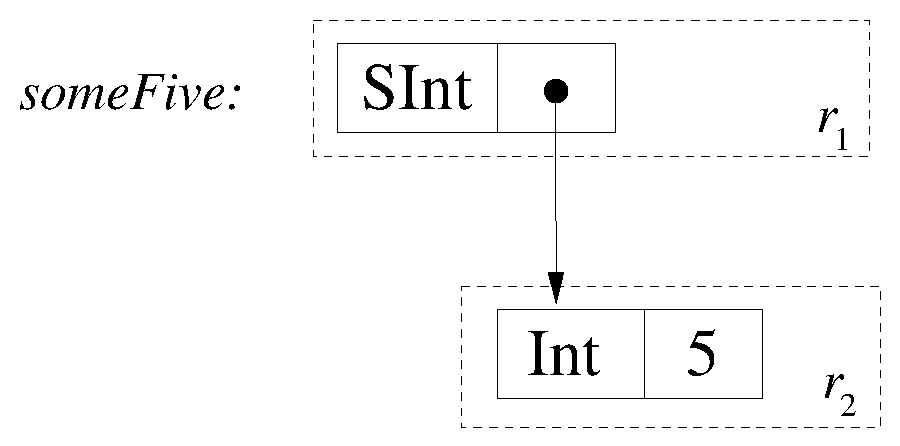
\includegraphics[scale=0.4]{2-System/fig/closure-someFive.eps}
\end{center}

As the outer constructor always appears in the primary region, the primary region variable is material. Because an $\iSInt$ object contains an $\iInt$ in a region named $r_2$, this variable is also material.

On the other hand, when we use $\iSFun$, the constructed object will contain a pointer to either the code for the function argument, or a thunk, depending on whether the argument was partially applied:

\begin{tabbing}
 	MMMMM \= MMMMMMMMMMM \= MMMMM \= MMMMMMMM \kill
	$\isomeSucc$ \> $= \iSFun \ \isucc$  \> $\isomeAdd$ \> $= \iSFun \ ((+) \ 2)$
\end{tabbing}

\vspace{-2em}
\begin{center}
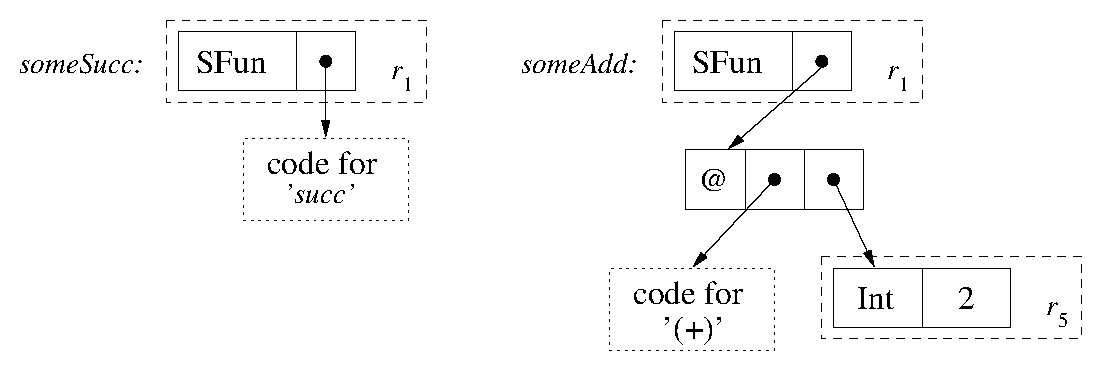
\includegraphics[scale=0.7]{2-System/fig/closure-someSuccAdd.eps}
\end{center}

Note that with the constructors at hand, there no way to create an $\iIntFun$ object that actually includes data in the $r_3$ or $r_4$ regions. Because of this, they are immaterial, and the generalisation of immaterial regions is not restricted as per the previous section. The type of $\isomeSucc$ above is:

\code{
	$\isomeSucc $
	& $::$		& \mc{3}{$\forall r_3 \ r_4 \ e_1. \ \iIntFun \ r_{1..4} \ e_1 \ \bot$} \\
	& $\rhd$ 	& $e_1$	& $\tme \iRead \ r_3$
}

Note that although our $\isomeSucc$ object does not include data in region $r_2$, that region is not quantified here. In general, if a particular value has type $\iIntFun \ r_{1..4} \ e_1 \ c_1$ then we will not know what data constructor was used to create it. We must rely on the data type definition to determine which regions are material.

The type of $\isomeAdd$ is similar, except that its closure variable is constrained to contain the type of the argument in the partial application of $(+)$:

\code{
	$\isomeAdd$ 
	& $::$		& \mc{2}{$\forall r_3 \ r_4 \ e_1 \ c_1. \ \iIntFun \ r_{1..4} \ e_1 \ c_1$} \\
	& $\rhd$	& $e_1$		& $\tme \iRead \ r_3 \lor \iRead \ r_5$ \\
	& $,$		& $c_1$		& $\tme \iInt \ r_5$
}

The material regions of a type are defined formally in \S\ref{inference:material-regions}.

\clearpage{}
% -----------------
\subsection{Strong, mixed and absent region variables}
\label{System:Closure:strong-mixed-absent-variables}

When an algebraic data type is defined we do not restrict the ways in which region variables are used. Due to this, a particular variable may occur in both a material and immaterial position. For example:

\code{
	\mc{4}{$\kdata \ \iIntFunMixed \ r_{1..5} \ e_1 \ c_1$} \\
	& $=$	& $\iSIntX$	& $(\iInt \ r_2)$ \\
	& $|$	& $\iSCharX$	& $(\iInt \ r_4)$ \\
	& $|$	& $\iSFunX$	& $(\iInt \ r_2 \lfuna{e_1 \ c_1} \iInt \ r_3)$
}

In the first constructor, $r_2$ is used as the primary region variable of $\iInt$, which makes it material. In the third constructor, $r_2$ is used as part of the type of a function parameter, so it is also immaterial. In this situation we say that $r_2$ is \emph{mixed material}.

If a region variable is \emph{only} ever used in a material position, then it is \emph{strongly material}. In the above definition, $r_1$ is strongly material because it is used as the primary region variable for $\iIntFunMixed$, and not in the type of a function parameter. The variable $r_4$ is also strongly material. We will use this concept when we discuss the polymorphic copy function in \S\ref{System:TypeClassing}. 

If a region variable is present as a parameter of the type constructor being defined, but not one of the data constructors, then we say it is \emph{absent}. The variable $r_5$ is absent in the above definition. As absent region variables cannot correspond to real regions in the store, all absent variables are also immaterial. The reverse is not true, as $r_3$ is immaterial, but not absent.


% --------------------
\subsection{Pure effects and empty closures}
\label{System:Closure:empty}
In the previous two sections, the definitions of $\iIntFun$ and $\iIntFunMixed$ include effect and closure variables as arguments to the type constructor. This allows these data types to be polymorphic in the effect and closure of the contained function. Alternatively, we could omit these variables as long as we constrained the types of $\iSFun$ and $\iSFunX$ so that the effect of the contained function was pure, and its closure contained no elements. 

A closure that has no elements is said to be \emph{empty}. Emptiness of closures is related to purity of effects. Recall from \S\ref{System:Effects:purification} that a pure effect is written $\bot$ and we can require an effect to be pure with the $\iPure$ constraint. Likewise, we write empty closures as $\bot$ and require a closure to be empty with the $\iEmpty$ constraint. We sometimes annotate $\bot$ with its kind, such as $\bot_{!}$ and $\bot_{\$}$ to distinguish between its two readings, but the kind is usually clear from context.

By omitting effect and closure variables, and restricting ourselves to a single region we will now define a diet version of $\iIntFun$ that has a single parameter instead of six. This new data type can still contain an $\iInt$ or function value, but the set of functions it could hold is reduced:

\code{
	\mc{4}{$\kdata \ \iIntFunDiet \ r_1$} \\
	& $=$	& $\iSIntD$	& $(\iInt \ r_1)$ \\
	& $|$	& $\iSFunD$	& $(\iInt \ r_1 \to \iInt \ r_1)$
}

\clearpage{}
\code{
	\mc{4}{$\kdata \ \iIntFunDiet \ r_1$} \\
	& $=$	& $\iSIntD$	& $(\iInt \ r_1)$ \\
	& $|$	& $\iSFunD$	& $(\iInt \ r_1 \to \iInt \ r_1)$
}

This modified data type definition generates the following constructors:

\code{
	$\iSIntD$ 
		& $::$ 	& $\forall r_1. \ \iInt \ r_1 \to \iIntFunDiet \ r_1$ 
	\\[1em]
	$\iSFunD$ 
		& $::$		& $\forall r_1 \ e_1 \ c_1$ \\
		& $.$	& $(\iInt \ r_1 \lfuna{e_1 \ c_1} \iInt \ r_1) \to \iIntFunDiet \ r_1$ \\
		& $\rhd $		& $\iPure \ e_1$ \\
		& $, $		& $\iEmpty \ c_1$ \\
}

Note that although $r_1$ is repeated in the first parameter of $\iSFunD$, this doesn't require its argument to be a function which simply passes the $\iInt$ through unchanged. The type of a function like $\isucc$ can be instantiated so that both its region variables are the same. Due to this we can still construct $(\iSFunD \ \isucc)$ as per the figure in \S\ref{System:Closure:non-material-regions}, though the single region will be forced $\iConst$ due to purification of the function's $\iRead$ effect. On the other hand, we can no longer construct $(\iSFunD \ ((+) \ 2))$ as its type would include a closure term due to the partial application, rendering it non-empty. See \S\ref{Evaluation:Limits:sharing-and-constraint-masking}
 for a possible way of addressing this limitation.

% --------------------
% \subsection{Shared regions which escape the analysis}
% Although closure typing goes a long way to model data sharing, inspection of the figures in the previous sections shows us that not all such data in the program is visible to the type system. In particular, the thunk created due to the partial application of $(+)$ in figure \ref{fig:typeSystem:uses-of-sfun} has not been assigned a region. 

% This is an important difference between our use of region variables and the way they are used in system such as MLKit\cite{tofte:mlkit-4.3.0}. In MLKit, \emph{all} data is assigned to a particular region, including thunks, which implies that function types are given region annotations as well \cite{tofte:region-inference}. In that system, regions are used for memory management whereas in ours they are used to identify non-interfering sets of computational effects, and to reason about mutability of data.

% \begin{itemize}
% \item	The lifetimes of thunks does not follow procedure activation closely. This is mentioned in MLKit paper about
% 	combining GC with region allocation.
% \item	We don't have region vars on function types, so we can't allocate them in regions, but we expect this not
% 	to be a problem.
% \item	Reference that paper on imperative data structures and the \texttt{close} operator.
% \end{itemize}


% --------------------
\subsection{Closure trimming}
\label{System:Closure:trimming}

The closure annotation attached to a function type lists the types of all free variables in that function's definition. However, not all of this information is useful to our analysis. As we only restrict the generalisation of material region variables, we only need to retain closure terms that contain them. The rest of the closure information can be trimmed out, and doing so is an important optimisation in practice.

Consider the following program:

\code{
	$x$ 		& 	& $= 5$			\\
 	$\ifun$		& ()  	& $= x + 1$ 		\\
 	$\ifunTwo$	& () 	& $= \ifun$  		\\
 	$\ifunThree$	& () 	& $= \ifunTwo$		\\
	$\ifunFour$	& () 	& $= \ifunThree$
}

This is a simple program, but as each successive binding refers to the binding above it, the closure terms in their types can become very large.

If $x$ has type $\iInt \ r_1$, then $\ifun$ has the following signature:

\code{
	$\ifun$ 
	& $::$		& $\forall r_2. \ () \lfuna{e_1 \ c_1} \iInt \ r_2$ \\
	& $\rhd$	& $e_1 = \iRead \ r_1$ \\
	& $,$		& $c_1 = x : \iInt \ r_1$
}

This says that $\ifun$ accepts a unit value and produces a freshly allocated integer. The closure constraint $c_1 = x : \iInt \ r_1$ says that the function refers to this object via the free variable $x$. When it evaluates, the addition operator reads the integer bound to $x$, hence the $\iRead \ r_1$ effect. It also reads the constant integer $1$, but as this constant is local to the function the effect is masked. 

\clearpage{}
Here is the type for $\ifunTwo:$

\qq\qq
\begin{tabular}{llllllll}
	$\ifunTwo$
	& $::$	& \mc{5}{$\forall r_2. \ () \lfuna{c_2} () \lfuna{e_1 \ c_1} \iInt \ r_2$} \\
	& $\rhd$& $e_1$	& \mc{3}{$= \iRead \ r_1$}	\\
	& $,$	& $c_1$	& \mc{3}{$= x : \iInt \ r_1$} 	\\
	& $,$	& $c_2$	& $= (\ifun$ 	& $:$	& \mc{2}{$\forall r_3. \ () \lfuna{e_3 \ c_3} \iInt \ r_3$} \\
	&	&	& 		& $\rhd$	& $e_3$		& $= \iRead \ r_1$ \\
	&	&	&	 	& $,$		& $c_3$		& $= x : \iInt \ r_1)$
\end{tabular}
\medskip

Note that $\ifunTwo$ refers to $\ifun$, so the full type of $\ifun$ appears in its closure. However, as we only use closure terms to reason about the sharing properties of data, we gain no benefit from carrying around information about the effects associated with a variable like $\ifun$. We also gain no benefit from retaining its argument and return types. We extend the concept of materiality to value types, and say that the argument and return positions of functions are immaterial because they do not represent objects in the store. Lastly, if we erase the return type $\iInt \ r_3$ then we do not need the quantifier $\forall r_3$. The only information about $\ifun$ that we \emph{do} need to keep is that it references a material object of type $\iInt \ r_1$. Using these observations we trim the type of $\ifunTwo$ to get:


\qq\qq
\begin{tabular}{llllllll}
	$\ifunTwo$
	& $::$	& \mc{5}{$\forall r_2. \ () \lfuna{c_2} () \lfuna{e_1 \ c_1} \iInt \ r_2$} \\
	& $\rhd$& $e_1$	& \mc{3}{$= \iRead \ r_1$}	\\
	& $,$	& $c_1$	& \mc{3}{$= x : \iInt \ r_1$} 	\\
	& $,$	& $c_2$	& $= \ifun : \iInt \ r_1$ 
\end{tabular}

Trimming closures prevents the types of functions from ``blowing up''. Without closure trimming the closure term of a top level function like $\imain$ would include all the types of all functions used in the program. In practice, most closure terms can be erased totally. For example, the definition of our $\iaddTwo$ function references the free variable $\isucc$. As $\isucc$ contains no material closure components, neither does $\iaddTwo$.

\code{
	\mc{2}{$\iaddTwo :: \forall r_1 \ r_2. \ \iInt \ r_1 \to \iInt \ r_2$} \\
	$\iaddTwo \ x$	& $= \isucc \ (\isucc \ x)$
}

In our current implementation we only trim out closure information concerning \emph{immaterial} region variables. Section \S\ref{Evaluation:Limits:sharing-and-constraint-masking} presents some ideas for also trimming out information concerning region variables that are constrained to be constant.

